\documentclass[
journal=jctcce,
layout=twocolumn
]{achemso}

\setkeys{acs}{
	abbreviations = false,
	articletitle  = false,
	keywords      = false,
	maxauthors    = 10,
	super         = true
}

% Comment below before submitting
\let\titlefont\undefined
\usepackage[fontsize=11pt]{scrextend}
\usepackage[hidelinks,colorlinks,citecolor=blue]{hyperref}
%\flushbottom
% Comment above before submitting
\usepackage{booktabs}
\usepackage{threeparttable}
\usepackage{amsmath}
\usepackage{amssymb}
\usepackage[T1]{fontenc}
\usepackage[table]{xcolor}
\definecolor{lightgray}{gray}{0.9}
\usepackage{tikz}
\usetikzlibrary{decorations.text}
\newcommand{\mt}[1]{\boldsymbol{\mathbf{#1}}}   % matrix symbol
\newcommand{\vt}[1]{\boldsymbol{\mathbf{#1}}}   % vector symbol
\newcommand{\tr}[1]{#1^\text{t}}                % transposition
\newcommand{\diff}[2]{\frac{\partial #1}{\partial #2}} % derivative
%\newcommand{\diff}[2]{\nabla_{#2}#1}            % derivative
\newcommand{\sdiff}[2]{\nabla^2_{#2}#1}         % 2nd derivative
\newcommand{\Ham}[1]{{\mathcal H}_\text{#1}}    % Hamiltonian
\newcommand{\Liu}[1]{i\!L_\text{#1}}            % Liouville
\newcommand{\timestep}{h}
\newcommand{\modified}[1]{\widetilde{#1}}

\usepackage{array}
\newcolumntype{L}{>{$}l<{$}}
\newcolumntype{C}{>{$}c<{$}}
\newcolumntype{R}{>{$}r<{$}}
\usepackage{booktabs}    
\usepackage[exponent-product=\times]{siunitx}

\newenvironment{smallarray}[1]                          % small arrays
{\null\,\vcenter\bgroup\scriptsize
	\renewcommand{\arraystretch}{1.5}
	\arraycolsep=.13885em
	\hbox\bgroup$\left[\array{@{}#1@{}}}
{\endarray\right]$\egroup\egroup\,\null}
\listfiles

\author{Ana J.
Silveira}
\email{asilveira@plapiqui.edu.ar}
\affiliation{Planta Piloto de Ingenier\'ia Qu\'imica, PLAPIQUI, Universidad Nacional del Sur, Camino La Carrindanga Km 7-CC: 717, Bah\'ia Blanca, Argentina}

\author{Charlles R.
A.
Abreu}
\email{abreu@eq.ufrj.br}
\affiliation{Chemical Engineering Department, Escola de Qu\'imica, Universidade Federal do Rio de Janeiro, Rio de Janeiro, RJ 21941-909, Brazil}

%\title{Revisiting the Nos\'{e}-Hoover chain thermostat for Rigid-Body Molecular Dynamics}
\title{Improvement of Deterministic NVT Molecular Dynamics via Backward Error Analysis}

%\abbreviations{AAA, BBB, CCC}
\keywords{aaa, bbb, ccc}

\begin{document}

\begin{tocentry}
	Graphical Abstract
\end{tocentry}

\begin{abstract}
	Abstract.
\end{abstract}

\section{Introduction}

Molecular Simulation, being the computational realization of Statistical Mechanics,\cite{Tuckerman_2010} involves several types of approximations in order to mimic ``real'' physical systems.
Naively, one would expect those approximations to only produce quantitative deviation from experimental values, and usually we tend to attribute any disagreement to a lack of accuracy of the force field.
However, what can be hidden in the deviations are actually systematic errors, which may introduce non-physical behaviour.
For instance, it has already been shown that the unavoidable truncation errors, associated with the numerical integration in Molecular Dynamics (MD), disrupt the equipartition of kinetic energy and, as a consequence, the temperature becomes an undefined property.\cite{Eastwood_2010} In a previous paper,\citep{Silveira_2017} we reported the same artifact to occur on the partition of kinetic energy between translational and rotational degrees of freedom in rigid-body MD.
That finding brings into question the method introduced by Kamberaj and co-workers\cite{Kamberaj_2005} which, assuming equipartition, couples separate chains of Nos\'{e}-Hoover thermostats on the rotational and translational degrees of freedom, but fails to reproduce the specified temperature for certain time step sizes.

The relevance of rigid-body MD stems from the fact that not only some molecules are modelled as rigid bodies, like the ubiquitous case of water,\cite{Jorgensen_1983} but also it is a simple coarse-graining strategy for systems that might be designed as collection of interconected rigid bodies, like proteins and nanoparticules.\cite{Knorowski_2012, Patra_2013} As a matter of fact, the approach of Kamberaj~\textit{et al.},\cite{Kamberaj_2005} which is implemented, for instance, in the softwares packages HOOMD-\textit{blue}\cite{Anderson_2008} and LAMMPS,\cite{Plimpton_1995} has been applied to simulate small molecules,\cite{Geiger_2013, Aimoli_2014, Aimoli_2014_2} as well as membranes,\cite{Bucior_2012} molecular motors,\cite{Akimov_2012} micelles\cite{Yan_2008} and nanoparticles.\cite{Patra_2014}

The Nos\'{e}-Hoover chain thermostat,\cite{Martyna_1992} routinely used in MD, is based on the extended phase-space approach that includes both the system of interest and extra degrees of freedom, which in turn are intended to control the kinetic energy fluctuations of the physical variables.
The dynamics of those extra degrees of freedom introduces non-Hamiltonian components to the equations of motion, with which backward error analysis is no longer feasible.
Altough it is not possible to devise symplectic integrators, one can rigurously obtain measure-preserving numerical solvers.\cite{Sergi_2001, Ezra_2004, Ezra_2006}

In this paper, we derive time reversible and measure-preserving numerical integrators for rigid-body MD in the canonical (NVT) ensemble.
The starting point is our previous work on the microcanonical (NVE) ensemble,\citep{Silveira_2017} which employs the unit quaternion representation for the rotational degrees of freedom.
Simultaneosuly coupling the translational and rotational degrees of freedom to a unique Nos\'{e}-Hoover chain thermostat, we are able to mantain the temperature of the system at its specified value.
The analysis of the integrators includes comparisons with results from the method introduced by Kamberaj~\textit{et al.},\cite{Kamberaj_2005} as well as with the Hybrid Monte Carlo (HMC) method,\cite{Duane_1987} which is exact in the sense that truncation errors do not affect its accuracy.
We also include results from simulations using the conventional SHAKE\cite{Ryckaert_1977} procedure, also coupled to a unique Nos\'{e}-Hoover chain.

backward error analysis

The paper is organized as follows.
In Sec.~\ref{sec:theory} we briefly review the equations of motion in the NVE ensemble, which are the basis for developing the corresponding dynamics in the NVT ensemble.
In Sec.~\ref{sec:numerical_solvers} we devise the corresponding numerical integrators, whose performance and correctness we assess in Sec.~\ref{sec:numerical_results}.
Finally, we present some concluding remarks in Sec.~\ref{sec:conclusion}.

\section{Methodology}
\label{sec:methodology}

\subsection{NVE Dynamics: Notation and Symplectic Integration}
\label{sec:nve}
In a previous paper \cite{Silveira_2017}, we took advantage of a particular factorization of the orientation matrix expressed in terms of quaternion components to
1) derive a new exact solution for torque-free rotations and use it as part of a symplectic numerical integrator for the motion of rigid bodies and
2) reinterpret the approximate NO-SQUISH method \cite{Miller_2002}, thus unveiling its equivalence to a method previously developed by Dullweber and co-workers \cite{Dullweber_1997}.

The Hamiltonian system of ordinary differential equations (ODE) that describes a rigid-body motion is given by \cite{Silveira_2017}
\begin{subequations}
	\label{eq:ODE system for NVE}
	\begin{align}
%
	&\dot{\vt r} =
	%+\diff{\Ham{}}{\vt p} =
	{\mt M}^{-1} {\vt p}, \\
%
	&\dot{\vt p} =
	%-\diff{\Ham{}}{\vt r} = 
	{\vt F}, \\
%
	&\dot{\vt q} =
	%+\diff{\Ham{}}{\vt \pi} =
	\frac{1}{2} \mt B(\vt q) \vt \omega, \text{ and} \label{eq:EDO_q} \\
%
	&\dot{\vt \pi} =
	%-\diff{\Ham{}}{\vt q} =
	\frac{1}{2} \mt B(\vt \pi) \vt \omega + 2 \mt C(\vt q) \vt \tau, \label{eq:EDO_pi}
	\end{align}
\end{subequations}
with $\vt \omega = \frac{1}{2} {\mt I}^{-1} \tr{\mt B}(\vt q) {\vt \pi}$.
In these equations, $\vt r$ is the center-of-mass position of the body, $\vt p$ is its linear momentum, $\vt q$ is a unit quaternion that determines its orientation, and $\vt \pi$ is the conjugated momentum of such quaternion.
Vectors $\vt F$ and $\vt \tau$ are, respectively, the resultant force and torque exerted on the body, both represented in the space-fixed frame of reference, while $\vt \omega$ is the three-dimensional angular velocity in the body-fixed frame.
Matrices $\mt M$ and $\mt I$ are diagonal ones.
The former contains the body mass in all three diagonal entries while the latter contains the three principal moments of inertia.
Finally, the matrix-valued functions $\mt B$ and $\vt C$ are defined as
\begin{equation*}
\label{eq:def_B_and_C}
\mt B(\vt q) = \begin{smallarray}{rrrr}
-q_2 & -q_3 & -q_4 \\
 q_1 & -q_4 &  q_3 \\
 q_4 &  q_1 & -q_2 \\
-q_3 &  q_2 &  q_1
\end{smallarray}
%
\; \text{and} \;
%
\mt C(\vt q) = \begin{smallarray}{rrrr}
-q_2 & -q_3 & -q_4 \\
 q_1 &  q_4 & -q_3 \\
-q_4 &  q_1 &  q_2 \\
 q_3 & -q_2 &  q_1
\end{smallarray}.
\end{equation*}

The factorization mentioned above, which played a central role in Ref.~\citenum{Silveira_2017}, is as simple as ${\mt A}(\vt q) = \tr{\mt B}(\vt q) {\mt C}(\vt q)$, with ${\mt A}(\vt q)$ being the orientation matrix of the body (that is, the rotation matrix connecting the body-fixed and space-fixed frames).

The Hamiltonian conserved by Eq.~\eqref{eq:ODE system for NVE} is
\begin{equation}
\label{eq:Hamiltonian}
\Ham{} = K(\vt p, \vt q, \vt \pi) + U(\vt r,\vt q),
\end{equation}
where $K$ and $U$ are the kinetic and potential energies of the body, respectively.
While $U(\vt r, \vt q)$ is an arbitrary function, the kinetic energy is given by
\begin{equation}
\label{eq:kinetic energy}
K = \frac{1}{2} \tr{\vt p} {\mt M}^{-1} {\vt p} + \frac{1}{8} \tr{\vt \pi} {\mt B}(\vt q) {\mt I}^{-1} \tr{\mt B}(\vt q) {\vt \pi}.
\end{equation}
%An advantage of this notation is that
Of course, Eqs.~\eqref{eq:ODE system for NVE} to \eqref{eq:kinetic energy} can also represent a system of $N$ interacting rigid bodies if we consider that vectors $\vt r$, $\vt p$, $\vt q$, and $\vt \pi$ contain the corresponding properties of all bodies piled together.
The same occurs for diagonal matrices $\mt M$ and $\mt I$, whose sizes increase to $3N \times 3N$ in this case.
In addition, $\mt B(\vt q)$ and $\mt C(\vt q)$ become block-diagonal matrices with $4N$ rows and $3N$ columns.
Yet, the notation can be made even more general if $\vt r$, $\vt p$, and $\mt M$ are enlarged further to accommodate a number of freely moving atoms.

A numerical solution of Eq.~\eqref{eq:ODE system for NVE} is usually represented by a stepwise application of the classical time-evolution propagator \cite{Tuckerman_2010} $e^{\timestep \Liu{\tiny NVE}}$ to the system configuration, where $\timestep$ is the time step size and $\Liu{\tiny NVE}$ is the Liouville operator associated to $\Ham{}$, which is
\begin{equation}
\label{eq:Lioville operator}
\begin{split}
\Liu{\tiny NVE} &= \tr{\vt p} {\mt M}^{-1} \diff{}{\vt r} + \frac{1}{2} \tr{\vt \omega} \tr{\mt B}(\vt q) \diff{}{\vt q} + \tr{\vt F} \diff{}{\vt p} \\
&+ \left[ \frac{1}{2} \tr{\vt \omega} \tr{\mt B}(\vt \pi) + 2 \tr{\vt \tau} \tr{\mt C}(\vt q) \right] \diff{}{\vt \pi}.
\end{split}
\end{equation}

A symplectic, time-reversible integrator can be devised by splitting the exponential operator according to the Trotter-Suzuki formula \cite{Trotter_1959, Suzuki_1976}
\begin{equation}
\label{eq:splitting NVE}
e^{\timestep \Liu{\tiny NVE}} = e^{\frac{\timestep}{2} \Liu{B}} e^{\timestep \Liu{A}} e^{\frac{\timestep}{2} \Liu{B}} + \mathcal{O}(\timestep^3),
\end{equation}
where $\Liu{A} + \Liu{B} = \Liu{\tiny NVE}$.
In the Verlet-type splitting of Ref.~\citenum{Silveira_2017}, the action of propagator $e^{\frac{\timestep}{2} \Liu{B}}$ is a kick in the linear and quaternion momenta given by ${\vt p} = {\vt p}^\ast + \frac{\timestep}{2} {\vt F}^\ast$ and ${\vt \pi} = {\vt \pi}^\ast + \timestep {\mt C}({\vt q^\ast}) {\vt \tau}^\ast$, respectively, where the asterisk denotes the state immediately before the propagation occurs.
The action of $e^{\timestep \Liu{A}}$ is the simultaneous uniform translation (${\vt r} = {\vt r}^\ast + \timestep {\mt M}^{-1} {\vt p}^\ast$) and torque-free rotation over a full time step. For this rotational part of the integration, in Ref.~\cite{Silveira_2017} we derived a general solution in a form that facilitates computer implementation and allows, differently to existing schemes \cite{Kosenko_1998,vanZon2007,Celledoni_2008}, a unified treatment for both asymmetric ($I_1$ $>$ $I_2$ $>$ $I_3$) and symmetric tops (either $I_1$ = $I_2$ or $I_2$ = $I_3$).
While the approximate solutions, such as the NO-SQUISH \cite{Miller_2002} method, only involve sine and cosine terms, the exact solution comprise ``less common'' functions, such as the Jacobi elliptic functions and Carlson integrals.
This contributes to the fact that the approximate solution is more commonly used \cite{vanZon2007}. 
For mathematical details, the reader is referred to our previos work \cite{Silveira_2017}, where we have verified that in liquid-phase simulations there is no significan gain in accuracy by using the exact solution in substitution to the NO-SQUISH as part of a symplectic integration scheme.
However, in the NO-SQUISH method an overall rotation is given by a sequence of uniform rotations around the principal axes of a body, which results in a factorization of the rotational operator given by $ e^{\frac{h}{2} i\!L_3} e^{\frac{h}{2} i\!L_2} e^{h i\!L_1} e^{\frac{h}{2} i\!L_2} e^{\frac{h}{2} i\!L_3}$, with each factor representing a rotation around a given axe. The analytical solution, on the other hand, entails a single operator, thus making the application of backward error analysis considerably simpler.

\subsection{NVT Dynamics with a Single Thermostat Chain}

Here we propose a new method for simulating a system of rigid bodies in the canonical ensemble.
For this, we couple a single Nos\'{e}-Hoover thermostat chain \cite{Martyna_1992} to all translational and rotational degrees of freedom of the rigid-body system.
This is simpler than the approach of Kamberaj \textit{et al}.,\cite{Kamberaj_2005} who employed separate thermostat chains to these two classes of movement.
To this end, we consider an extra generalized coordinate $\eta_j$ and its conjugate momentum $p_{\eta_j}$ for each thermostat $j$, with $1 \leq j \le M$.
The flow in the extended phase-space no longer conserves the Hamiltonian $\Ham{}$, but an ``extended energy'' given by \cite{Martyna_1992}
\begin{equation}
\label{eq:nvt extended energy}
H = K + U + {\textstyle\sum\limits_{j=1}^{M}} \frac{p_{\eta_j}^2}{2Q_j} + L k_\text{\tiny B} T\eta_1 + k_\text{\tiny B} T {\textstyle\sum\limits_{j=2}^{M}} \eta_j,
\end{equation}
where $k_\text{\tiny B}$ is the Boltzmann constant, $T$ is the system temperature, $L$ is a constant to be determined, and each $Q_j$ is an inertial parameter.
As recommended in Ref.~\citenum{Martyna_1992}, we can make $Q_1 = L k_\text{\tiny B} T t_d^2$ and $Q_j = k_\text{\tiny B} T t_d^2$ for $j \geq 2$, where $t_d$ is a characteristic time scale of the thermostat chain.

Knowledge on the dynamics and statistical mechanics of non-Hamiltonian systems has advanced considerably in recent years.\cite{Tuckerman_1999, Tuckerman_2001, Sergi_2001, Sergi_2003, Ezra_2004, Sergi_2004, Ezra_2006, Sergi_2010_2} Invaluable tools have been devised for the development and analysis of extended phase space methods.
By employing the method of Sergi and Ferrario \cite{Sergi_2001}, we obtain the equations of motion for the NVT dynamics with a single thermostat chain, which are
\begin{subequations}
	\label{eq:ODE system for NVT}
	\begin{align}
%
\label{eq:nhc_r}
	&\dot{\vt r} =
	{\mt M}^{-1} {\vt p}, \\
%
\label{eq:nhc_p} 
	&\dot{\vt p} =
	{\vt F} - \alpha_1 {\vt p},\\
%
\label{eq:nhc_q}
	&\dot{\vt q} =
	\frac{1}{2} \mt B(\vt q) \vt \omega, \\
%
\label{eq:nhc_pi}
	&\dot{\vt \pi} =
	\frac{1}{2} \mt B(\vt \pi) \vt \omega + 2 \mt C(\vt q) \vt \tau - \alpha_1 {\vt \pi}, \\
%
\label{eq:nhc_eta}
	&\dot{\eta}_j = \alpha_j, \text{ and} \\
%
\label{eq:nhc_p_eta}
	&{\dot p}_{\eta_j} = G_j - \alpha_{j+1} p_{\eta_j} \qquad \text{for} \quad 1 \leq j \le M.
	\end{align}
\end{subequations}

In these equations, $\alpha_j$ $=$ ${p_{\eta_j}}/{Q_j}$ for $1 \leq j \le M$ and $\alpha_{M+1} = 0$, while $G_j$ is a generalized force acting on thermostat $j$, defined as
\begin{subequations}
\begin{align}
\label{eq:generalized force NVT}
&G_1 = \tr{\vt p} \diff{K}{\vt p} + \tr{\vt \pi} \diff{K}{\vt \pi} - L k_\text{\tiny B} T \quad \text{and}\\
&G_j = \frac{p_{\eta_{j-1}}^2}{Q_{j-1}} - k_\text{\tiny B} T  \qquad \text{for} \quad j > 1.
\end{align}
\end{subequations}

With $K$ defined as in Eq.~\eqref{eq:kinetic energy}, it turns out that $G_1 = 2K - L k_\text{\tiny B} T$.
It is worth noting that the $\eta$ coordinates are driven variables with no influence on the dynamics, but are often computed for checking how well a numerical integrator conserves $H$.
Analysis of the probability distribution generated by Eq.~\eqref{eq:ODE system for NVT} can be done through the generalized phase-space analysis of Tuckerman \textit{et al}.\cite{Tuckerman_2001} For this, conservation laws must be identified and driven variables eliminated.
If there are no external forces, the vector quantity $e^{\eta_1}\sum_{i=1}^N {\vt p}_i$ and the extended energy $H$ are integrals of motion, while the system's center-of-mass position can be considered as a driven variable,\cite{Tuckerman_2001} such as the $\eta$ coordinates.
Moreover, $2N$ equations must be eliminated due to the constraints involving $\vt q$ and $\vt \pi$.
In the general case, by taking all these facts into account and applying the analysis of Ref.~\citenum{Tuckerman_2001}, we can deduce that the correct canonical distribution is attained if one makes $L = 6N$.
In the particular situation in which one sets $\sum_{i=1}^N {\vt p}_i = \vt 0$ at the onset of a simulation, one must make $L = 6N - 3$ \cite{Martyna_1994}.

\subsection{Measure-Preserving Integration for the NVT Dynamics}
\label{sec:mttk}
As in the Hamiltonian case, it is possible to devise a splitting scheme for solving Eq.~\eqref{eq:ODE system for NVT} numerically \cite{Tuckerman_2010}. For that, we employed the systematic method introduced by Ezra \cite{Ezra_2006} for deriving accurate integrators which preserve the phase-space measure associated with the original equations of motion, which is 
In short, a splitting scheme will preserve a given measure if each individual propagator does it as well. 
It can be shown that the function $w(\vt x)$ that determines the invariant phase-space measure is given by
\begin{equation}
\label{eq:nhc_measure}
w = -7N \eta_1 - \sum_{j=2}^M \eta_j.
\end{equation}

will preserve a given measure $e^{-w(\vt x)}d\vt x$ 

By defining a propagator $e^{\timestep \mathcal{L}_\text{\tiny NVT}}$, where $\mathcal{L}_\text{\tiny NVT}$ is a generalized (i.e.
non-Hamiltonian) Liouville operator, the splitting goes as
\begin{equation}
\label{eq:splitting NVT}
e^{\timestep \mathcal{L}_\text{\tiny NVT}} = e^{\frac{\timestep}{2} \mathcal{L}_\text{\tiny NHC}} e^{\timestep \Liu{\tiny NVE}} e^{\frac{\timestep}{2} \mathcal{L}_\text{\tiny NHC}} + \mathcal{O}(\timestep^3),
\end{equation}
where $\Liu{\tiny NVE}$ is the same operator of the previous case and $\mathcal{L}_\text{\tiny NHC}$ aggregates all new terms introduced by the Nos\'e-Hoover chain.
Of course, the NVE part can be integrated exactly as described before.
The NHC part, in turn, can be split even further as
\begin{equation*}
e^{\frac{\timestep}{2} \mathcal{L}_\text{NHC}} = \left[ \left( \textstyle\prod\limits_{j=M}^1 e^{\frac{\timestep}{4n} \mathcal{L}_j }\right) e^{\frac{\timestep}{2n} \mathcal{L}_0 } \left(  \textstyle\prod\limits_{j=1}^M e^{\frac{\timestep}{4n} \mathcal{L}_j }\right)  \right]^n.
\end{equation*}

In the scheme above, the first propagator to act is $e^{\frac{\timestep}{4n} \mathcal{L}_M}$, which promotes a kick in the momentum of thermostat $M$ expressed as $p_{\eta_M} = p_{\eta_M}^\ast + G_M^\ast \frac{\timestep}{4n}$.
Then, propagators $e^{\frac{\timestep}{4n} \mathcal{L}_j}$ act sequentially, with $j$ varying from $M-1$ down to $1$.
With $\phi(x) = \frac{1-e^{-x}}{x}$, the effect of each one is translated as \cite{Martyna_1996}
\begin{align*}
&p_{\eta_j} = p_{\eta_j}^\ast + \Big( G_j^\ast - \alpha_{j+1}^\ast p_{\eta_j}^\ast \Big) \phi\left(\frac{\alpha_{j+1}^\ast \timestep}{4n}\right) \frac{\timestep}{4n} \; \text{and} \\
&\eta_{j+1} = \eta_{j+1}^\ast + \alpha_{j+1}^\ast \frac{\timestep}{4n}.
\end{align*}

After that, propagator $e^{\frac{\timestep}{2n} \mathcal{L}_0}$ establishes the effect of thermostat $1$ on the motion of the rigid bodies, as well as the evolution of coordinate $\eta_1$.
Its action is expressed as ${\vt p} = e^{-\alpha_1^\ast \frac{\timestep}{2n}} {\vt p}^\ast$, ${\vt \pi} = e^{-\alpha_1^\ast \frac{\timestep}{2n}} {\vt \pi}^\ast$, and $\eta_1 = \eta_1^\ast + \alpha_1^\ast \frac{\timestep}{2n}$.
Finally, propagators $e^{\frac{\timestep}{4n} \mathcal{L}_j}$ are applied once again, but now with index $j$ ascending from $1$ to $M$.
In the following, the NVT integrator introduced in the present section will be denoted as MTTK as its development was inspired by Ref.~\cite{Martyna_1996}.

For having a low computational cost, the whole procedure described above can be repeated $n$ times with little impact on the overall integration effort, making it feasible to increase the time step $\timestep$ without degrading the accuracy of the NHC part.
In contrast, evaluating the NVE part is expensive for involving force/torque computations and, in addition, its accuracy goes down very quickly as $\timestep$ increases \cite{Davidchack_2010, Silveira_2017}.
A high-order integration scheme\cite{Omelyan_2007, Van_zon_2008} could possibly admit larger time steps, but it would raise both cost and complexity for entailing the computation (or numerical estimation) of force/torque gradients.
The processed splitting approach \cite{Omelyan_2008} seems promising, but its extension to the NVT case without doing back-and-forth processing at every time step would require further theoretical development.
Here we choose to take a simpler path.
Instead of trying to increase accuracy in the evaluation of $e^{\timestep \Liu{\tiny NVE}}$, we attempt to quantify the implied deviations, with which we can both tune the thermostatting procedure and properly weight the sampled configurations when computing ensemble averages.

\subsection{Backward Error Analysis}
\label{sec:modified_h}

In order to explain our proposal, we turn the attention again to the NVE case.
A known property of splitting methods applied to Hamiltonian ODE systems is that they provide approximate solutions which are Hamiltonian as well.
Hence, a trajectory generated to be roughly consistent with the specified function $\Ham{}$ will be exactly consistent with a nearby (albeit unknown) function $\Ham{S}$, referred to as a shadow Hamiltonian \cite{Hairer_2006}.
In this way, while $\Ham{}$ exhibits a certain degree of oscillation along that trajectory, the value of $\Ham{S}$ is actually conserved (up to round-off errors). 
It is also known that $\Ham{S}$ explicity depends on the time step size $\timestep$.

The first new result we present in this paper is an analytical form for the shadow Hamiltonian concerning a system of rigid bodies whose dynamics is integrated via the unsplit rotation method of Ref.~ \citenum{Silveira_2017}.
A detailed derivation is provided in Appendix~\ref{sec:rigid body shadow hamiltonian} and here we summarize the final expressions.

As shown in Appendix~\ref{sec:rigid body shadow hamiltonian}, the shadow Hamiltonian for a Verlet-type method applied to a system of rigid bodies can be approximated by $\Ham{S} = \modified K + \modified U + \mathcal{O}(h^4)$, where $\modified K$ and $\modified U$ are modified kinetic and potential energies.
The latter is given by
\begin{equation}
\label{eq:modified potential energy}
\modified U = U - \frac{\timestep^2}{24} \left( \tr{\vt F} {\mt M}^{-1} {\vt F} + \tr{\vt \tau}_b {\mt I}^{-1} {\vt \tau}_b \right),
\end{equation}
where ${\vt \tau}_b = {\mt A}(\vt q) {\vt \tau}$ is the body-fixed representation of the resultant torque vector.
Note that $\modified U$, such as $U$, is independent of $\vt p$ and $\vt \pi$.
In turn, the modified kinetic energy can be expressed as
\begin{equation}
\label{eq:modified kinetic energy}
\modified K = \frac{1}{2} \tr{ \left[\begin{array}{c} \vt p \\ \vt \pi \end{array}\right]} \modified{\mathbf \Omega}(\vt r, \vt q, \timestep^2) \left[\begin{array}{c} \vt p \\ \vt \pi \end{array}\right],
\end{equation}
where $\modified{\mathbf \Omega}$ is a symmetric matrix-valued function of $\vt r$, $\vt q$, and $\timestep^2$, given by $\tilde{\mt \Omega} = {\mt \Omega} + {\timestep^2}/{6} \left( {\mt \Omega} {\mt U}_{\vt x \vt x} \tr{\mt \Omega} \right)$, where
\begin{equation*}
{\mt \Omega} = \left[\begin{array}{cc}
{\mt M}^{-1} & \mt 0 \\
\mt 0 & \frac{1}{4} {\mt B}(\vt q) {\mt I}^{-1} \tr{\mt B}(\vt q)
\end{array}\right]
\end{equation*}
and ${\mt U}_{\vt x \vt x}$ is the Hessian matrix of the potential energy with respect to the entries of $\vt r$ and $\vt q$, given by
\begin{equation*}
{\mt U}_{\vt x \vt x} = \left[\begin{array}{cc}
U_{\vt r \vt r} & U_{\vt r \vt q} \\
U_{\vt q \vt r} & U_{\vt q \vt q}
\end{array}\right].
\end{equation*}

Hence, the trajectory generated by the splitting scheme of Eq.~\ref{eq:splitting NVE}, which is intended to approach the exact solution of Eq.~\eqref{eq:ODE system for NVE}, will approach even more closely the solution of a modified ODE system given by
\begin{equation*}
\dot{\vt r} = \diff{\modified K}{\vt p}, \;
\dot{\vt q} = \diff{\modified K}{\vt \pi}, \;
\dot{\vt p} = -\diff{\modified{\Ham{}}}{\vt r}, \; \text{and} \;
\dot{\vt \pi} = -\diff{\modified{\Ham{}}}{\vt q}.
\end{equation*}

The first two of these equations can be combined together so that we can use Eq.~\eqref{eq:modified kinetic energy} to obtain
\begin{equation}
\label{eq:shadow ODE system}
\left[\begin{array}{c} \dot{\vt r} \\ \dot{\vt q} \end{array}\right] = \modified{\mathbf \Omega}(\vt r, \vt q, \timestep^2) \left[\begin{array}{c} \vt p \\ \vt \pi \end{array}\right].
\end{equation}

Analytical calculation of $\modified U$ via Eq.~\eqref{eq:modified potential energy} is straightforward.
In contrast, although it is possible to compute $\modified K$ by direct evaluation of Eq.~\eqref{eq:modified kinetic energy}, this is a complex and expensive task.
Fortunately, we can estimate it rather easily though a method devised by \citeauthor{Eastwood_2010} \cite{Eastwood_2010}, which consists in using numerical differentiation to estimate the time-derivatives $\dot{\vt r}$ and $\dot{\vt q}$ directly from the obtained NVE trajectory.
Considering $n$-th order estimators $\dot{\vt r}^{[n]}$ and $\dot{\vt q}^{[n]}$, we substitute Eq.~\eqref{eq:shadow ODE system} into Eq.~\eqref{eq:modified kinetic energy} to find out that
\begin{equation}
\label{eq:modified kinetic energy estimator}
\modified K = \frac{1}{2} \left( \tr{\vt p} \dot{\vt r}^{[n]} + \tr{\vt \pi} \dot{\vt q}^{[n]} \right) + \mathcal{O}(h^n).
\end{equation}

For reasons that will become clear shortly, we employ an asymmetric, four-point stencil formula for estimating $\dot{\vt r}$ at a given instant $t$, which is
\begin{equation*}
\dot{\vt r}^{[3]}_t = \frac{{\vt r}_{t-2\timestep} - 6 {\vt r}_{t-\timestep} + 3 {\vt r}_t + 2 {\vt r}_{t+\timestep}}{6\timestep}.
\end{equation*}

In the case of quaternions, as a simple polynomial interpolation is insufficient to ensure that $\tr{\vt q}_i \dot{\vt q}_i = 0$ at all times for each rigid body $i$, such as required for satisfying the unit-norm condition \cite{Silveira_2017}, we estimate the time-derivative $\dot{\vt q}$ by means of\cite{Schay_1995}
\begin{equation*}
\dot{\vt q}^{[3]}_t = {\mt \Pi}({\vt q}_t) \frac{{\vt q}_{t-2\timestep} - 6 {\vt q}_{t-\timestep} + 3 {\vt q}_t + 2 {\vt q}_{t+\timestep}}{6\timestep},
\end{equation*}
where ${\mt \Pi}$ is a matrix-valued function given by either product ${\mt B}\tr{\mt B}$ or ${\mt C}\tr{\mt C}$ \cite{Silveira_2017}.
In practice, we evaluate the equation above individually for each body $i$ with ${\mt \Pi}({\vt q}_i) = {\mt 1} - {\vt q}_i \tr{\vt q}_i$, where $\mt 1$ is the identity matrix, thus projecting the interpolation-based derivative quaternion into the hyperplane orthogonal to ${\vt q}_i$.

\subsection{Adjustment of the NVT Dynamics}
\label{sec:smttk}
Bringing the attention back to the NVT case, our proposal consists in acknowledging that the middle propagator in Eq.~\eqref{eq:splitting NVT}, if split according to Eq.~\eqref{eq:splitting NVE}, produces a phase-space move that is more consistent with the modified Hamiltonian ODE system than with the original one.
Thus, we should adjust the Nos\'e-Hoover chain so as to provide a distribution proportional to $e^{-\beta \modified{\Ham{}}}$ rather than $e^{-\beta \Ham{}}$, where $\beta = \frac{1}{k_\text{\tiny B} T}$.
Fortunately, this entails solving Eq.~\eqref{eq:ODE system for NVT} almost exactly, by means of splitting scheme, as described before.
The only required modification is that $\modified K$ replaces $K$ in Eq.~\eqref{eq:generalized force NVT}, which defines the force $G_1$.
By contrasting such definition with Eqs.~\eqref{eq:modified kinetic energy} and \eqref{eq:shadow ODE system}, we observe that $G_1$ becomes
\begin{equation}
\label{eq:thermostat_force}
G_1 = 2 \modified K - L k_\text{\tiny B} T.
\end{equation}

One instant in which $\modified K$ must be evaluated is right after the action of propagator $e^{\timestep \Liu{\tiny NVE}}$.
Notice that such action takes place only once per time step, intercalating with non-Hamiltonian propagations.
Therefore, there is no record beforehand of a Hamiltonian trajectory from which we can estimate $\dot{\vt r}^{[n]}$ and $\dot{\vt q}^{[n]}$ with high accuracy.
This could be solved by executing a number of virtual Verlet steps, both forward and backward in time, so as to generate a virtual Hamiltonian trajectory that coincides with the actual trajectory in the two phase-space points which are input and output of the central propagator in Eq.~\eqref{eq:splitting NVT}.
Nonetheless, this might require additional force computations per actual time step, thus increasing the cost of the simulation.
Fortunately, only positions and orientations are required for the numerical differentiation.
This allows us to obtain a four-point stencil without any additional force evaluation, just by executing one incomplete virtual step for each direction in time.
By incomplete we mean that the step is aborted once the positions and orientations have been updated.
\begin{figure}
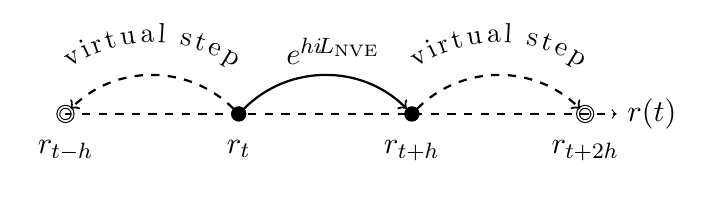
\begin{tikzpicture}
%\draw[dash pattern=on 2pt off 3pt on 4pt off 4pt](3,.2) -- (3,1.5);
%\draw[dash pattern=on 2pt off 3pt on 4pt off 4pt](5.5,.2) -- (5.5,1.5);
\draw[->, dashed]   (0,0.0) -- (7,0.0) node[right]{$r(t)$};
\node(0) at (0,0)[shape=circle,draw,double,scale=0.5]        {};
\node(1) at (2.2,0)[fill=black,shape=circle,draw,scale=0.5]        {};
\node(2) at (4.4,0)[fill=black,shape=circle,draw,scale=0.5]        {};
\node(3) at (6.6,0)[shape=circle,draw,double,scale=0.5] {};
\node(4) at (3.4,0.8)[] {$e^{\timestep \Liu{\tiny NVE}}$};
\node at (0.0,-0.2)[below]{$r_{t-h}$};
\node at (2.2,-0.2)[below]{$r_{t}$};
\node at (4.4,-0.2)[below]{$r_{t+h}$};
\node at (6.6,-0.2)[below]{$r_{t+2h}$};
\path[->,thick] (1) edge [bend left=45] (2);
\path[dashed,->,thick,postaction={decorate,decoration={raise=2.5ex,text along path,text align=center,text={|\small|virtual step}}}] (0) to [bend left=45] (1);
\path[dashed,->,thick] (1) edge [bend right=45] (0);
\path[dashed,->,thick,postaction={decorate,decoration={raise=2.5ex,text along path,text align=center,text={|\small|virtual step}}}] (2) to [bend left=45] (3);
\path[dashed,->,thick] (2) edge [bend left=45] (3);
\end{tikzpicture}
\caption{Schematic representation}
\label{fig:virtual}
\end{figure}
%\begin{figure}
%\begin{tikzpicture}
%\draw[dash pattern=on 2pt off 3pt on 4pt off 4pt](2,.2) -- (2,1.5);
%\draw[dash pattern=on 2pt off 3pt on 4pt off 4pt](5.5,.2) -- (5.5,1.5);
%\node(0) at (0,0)[shape=circle,draw, minimum width=1cm, minimum height=1cm]        {$r_{t-h}$};
%\node(1) at (2.5,0)[shape=circle,draw,double,minimum width=1cm, minimum height=1cm]        {$r_t$};
%\node(2) at (5,0)[shape=circle,draw,double,minimum width=1cm, minimum height=1cm]        {$r_{t+h}$};
%\node(3) at (7.5,0)[shape=circle,draw,minimum width=1cm, minimum height=1cm] {$r_{t+ 2h}$};
%\node(4) at (3.75,1)[] {$e^{\timestep \Liu{\tiny NVE}}$};
%\path [dashed,->]
%  (1)      edge                 node [above]  {virtual}     (0)
%  (2)      edge                 node [above] {virtual}     (3);
%\path [->,thick] 
%  (1)      edge                 node [above]  {}            (2);
%\end{tikzpicture}
%\caption{Schematic representation}
%\label{fig:virtual}
%\end{figure}

A drawback of this approach is that the resulting NVT integrator lacks time-reversal symmetry due to the employed differentiation formulas.
As a matter of fact, long-term reversibility is not generally achievable with MD codes that rely on floating-point arithmetics.
In any event, if short-term reversibility is a requirement, one can simply employ a symmetric five-point stencil formula, at the price of one additional force computation round per actual time step.

In addition, $\modified K$ must be reevaluated after the action of propagator $e^{\frac{\timestep}{2n} {\mathcal L}_0}$, which scales the momentum vectors $\vt p$ and $\vt \pi$ by a common factor $e^{-\alpha_1^\ast \frac{\timestep}{2n}}$.
Because such propagator leaves the positions and quaternions intact and, as a consequence, the matrix $\modified{\mathbf \Omega}(\vt r, \vt q, \timestep^2)$ in Eq.~\eqref{eq:modified kinetic energy} remains unaltered, the reevaluation of $\modified K$ goes as simply as ${\modified K} = e^{-\alpha_1^\ast \frac{\timestep}{n}} {\modified K}^\ast$.

$\widetilde{H}$, but an ``extended energy'' given by \cite{Martyna_1992}
\begin{equation}
\label{eq:this extended energy}
\widetilde{H} = \modified K + \modified U + {\textstyle\sum\limits_{j=1}^{M}} \frac{p_{\eta_j}^2}{2Q_j} + L k_\text{\tiny B} T\eta_1 + k_\text{\tiny B} T {\textstyle\sum\limits_{j=2}^{M}} \eta_j,
\end{equation}

Tolman's generalized equipartition theorem \cite{Uline_2008}
\begin{equation*}
\left\langle \tr{\vt p} \diff{\modified{\Ham{}}}{\vt p} + \tr{\vt \pi} \diff{\modified{\Ham{}}}{\vt \pi} \right\rangle = (6N - 3) k_\text{\tiny B} T
\end{equation*}


Finally, reweighting:
\begin{equation}
\label{eq:reweighting}
\langle A \rangle = \frac{\sum\limits_{i=1}^{N_s} A(\vt x_i) \exp \left[{\frac{\modified{\Ham{}}(\vt x_i) - {\Ham{}}(\vt x_i)}{k_\text{\tiny B} T}}\right]}{\sum\limits_{i=1}^{N_s} \exp \left[{\frac{\modified{\Ham{}}(\vt x_i) - {\Ham{}}(\vt x_i)}{k_\text{\tiny B} T}}\right] }.
\end{equation}

\section{Theoretical Background}


We remark that the integration scheme proposed by Kamberaj \text{et al}.\cite{Kamberaj_2005} does not fulfill this criterion. 

We end this section by noting that the term that premultiplies the extended phase-space volume in the invariant-measure above is a function of $\vt \eta$. Given that the time evolution of the physical variables and the thermostat momenta does not depend on $\vt \eta$, we might conclude that, in this case, the measure-preserving condition for every individual operator can actually be relaxed. However, as will be shown in the numerical results of Sec.~\ref{sec:numerical_results}, 


\subsection{Generalized Equipartition}

The important thing is that $\modified{\mathbf \Omega}$ depends exclusively on the positions and orientations, which makes $\left[\begin{array}{c} \diff{\modified K}{\vt p} \\ \diff{\modified K}{\vt \pi} \end{array}\right] = \modified{\mathbf \Omega} \left[\begin{array}{c} \vt p \\ \vt \pi \end{array}\right]$.
In this way, the equipartition theorem (valid at least in this direction? something to do with integrating through momenta at least internally to the integral in coordinates?) states that
\begin{equation}
\label{eq:equipartition}
3N k_B T = \left\langle \tr{\vt p} \diff{\tilde K}{\vt p} \right\rangle = 2\langle \tilde K \rangle
\end{equation}

Sampling validation: Shirts \cite{Shirts_2013}

\section{Results}
\label{sec:numerical_results}

In the following, we analyze the performance of the proposed NVT integrators introduced in Secs. \ref{sec:mttk}-\ref{sec:smttk}, and  compare the results with those obtained employing the method of Kamberaj \textit{et al.} \cite{Kamberaj_2005}. 
The system under study corresponds to 903 TIP3P\cite{Jorgensen_1983} water molecules at a density of 970 kg/m$^3$.
The 12-6 Lennard-Jones and damped Coulombic interactions were truncated at  10 {\AA} and smoothed via a switching function over the range of 9.5 {\AA} to  10 {\AA}.\cite{Silveira_2017} 
The damping of Coulombic interactions was done by a factor erfc($\alpha r$), with $\alpha$ = 0.29 {\AA}$^{-1}$.

Before showing our main results, it may be instructive first to give a picture of the problem in controlling the temperature when discretization errors are non-negligible. 
The most direct way (the most senstive indicator of the presence of discretization errors) to determine the importance of these errors is by examining the departure of the ``modified Hamiltonian'' $\modified{\Ham{}}$ from the physical Hamiltonian $\Ham{}$\cite{Engle_2005}. 
Fortunately, with the analytical form of $\modified{\Ham{}}$ derived in this paper we are able to perform such an analysis for the NVE integrator which is essential, as will be shown below, to understand the results of the NVT methods. 
In Fig.~\ref{fig:nve} we depict the time evolution of both $\modified{\Ham{}}$ (dotted lines) and $\Ham{}$ (solid lines) for the water system undergoing NVE dynamics with different step sizes ($\timestep$).
The numerical integrator correspons to Eq.~\ref{eq:splitting NVE} with the exact solution of free rotation. 
As expected, $\modified{\Ham{}}$ is very well conserved and close to $\Ham{}$ for $\timestep$ fs, but fairly rapidly separates from $\Ham{}$ when increasing $\timestep$. 
It should be remarked that $\modified{\Ham{}}$ corresponds to a simple approximation and, most important, it is computationally very cheap. As a result of employing such approximation, we have larger fluctuations in $\modified{\Ham{}}$ for $\timestep$ fs and $\timestep$ fs (add in conclusions that we should use high-order approximations).

\begin{figure}
	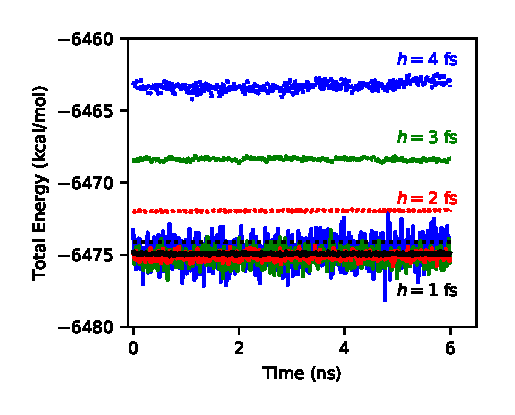
\includegraphics{Figures/NVE.eps}
	\caption{Total energy $\Ham{}$ (solid lines) and modified Hamiltonian $\modified{\Ham{}}$ (dotted lines) of 903 TIP3P\cite{Jorgensen_1983} water molecules obtained by NVE MD simulations for different step sizes $\timestep$. The numerical integrator correspons to Eq.~\ref{eq:splitting NVE} with the exact solution of free rotation.}
	\label{fig:nve}
\end{figure}

For our implementation for rigid bodies of the numerical scheme due to Martyna \textit{et al.} \cite{Martyna_1996} (Eq.~\ref{eq:splitting NVT}), in Fig.~\ref{fig:props_k_m} we depict the computed averages of temperature ($\langle T \rangle$) and potential energy per molecule ($\langle U \rangle$) as a function of $\timestep$. 
The specified temperature corresponds to T = 298 K.
Fig.~\ref{fig:props_k_m} clearly shows that a suitable temperature control leads to a severely degraded accuracy in $\langle U \rangle$, which systematically increases with $\timestep$.
As demonstrated in Fig.~\ref{fig:nve}, the discretization errors are non-negligible even for a small step size of 2 fs.
Thus, the results of Fig.~\ref{fig:props_k_m} can be interpreted as follows: if the kinetic energy is restricted to adopt a certain value, in accordance with the specified temperature, the unavoidable discretization errors will accumulate in the remaining degrees of freedom.
These observations motivated the development of the scheme of Sec.~\ref{sec:smttk}, whose promising results we show below.

\begin{figure}
	\includegraphics{Figures/thermodynamic_properties_intro.eps}
    \caption{Effect of the time-step size on the thermodynamic properties and of 903 TIP3P\cite{Jorgensen_1983} water molecules in NVT MD simulations employing...}
	\label{fig:props_k_m}
\end{figure}

\subsection*{Numerical Stability}

First, we report related the numerical stability of the NVT integrators.


examine the numerical stability of the NVT integrators by simply monitoring the quantity expected to be conserved along the simulation in each case: $\widetilde{H}$ (Eq.~\ref{eq:this extended energy}) for the proposed method, and $H$ (Eq.~\ref{eq:nvt extended energy}) for the integrators due to Martyna \textit{et al.} \cite{Martyna_1996} and Kamberaj \textit{et al.} \cite{Kamberaj_2005}.
In Table~\ref{table:stability} we report the energy drift, denoted by $R$, as the the rate of change of $\widetilde{H}$ (kcal/mol) with time (ns), which is the angular coefficient obtained from linear regression fitting between those variables. As it is already known that \cite{Davidchack_2009,Bond_2007}

we plot these extended energies for different time step sizes. From Figs.~\ref{fig:num_stab}(a) and (b) which, respectively, correspond to the integrator proposed in this work and our implementation of the scheme due to Martyna \textit{et al.} \cite{Martyna_1996}, one notes that the energy appears to remain bounded for time step sizes up to 5 fs, and a continous drift takes place for $\timestep$ = 6 fs. The numerical stability is only modestly improved by our method.
The result that stands out, because of its anomalous feature, corresponds to Fig.~\ref{fig:num_stab} (c), which was obtained employing the method of Kamberaj \textit{et al.} \cite{Kamberaj_2005}.
Note that for each time step size, the extended energy continously increases until reaching a point at which the integrator becomes stable.
It should be remarked that these results were double-checked with the LAMMPS software package \cite{Plimpton_1995}. 
As already mentioned, the scheme due to Kamberaj \textit{et al.} \cite{Kamberaj_2005} couples separate chains of Nos\'{e}-Hoover thermostats on the rotational and translational degrees of freedom.
Davidchack \cite{Davidchack_2009} also implemented such a separate thermostatization and discovered the existance of energy flows from one thermostat to the other.
To the best of our knowledge, the work of Davidchak \cite{Davidchack_2009} did not result in a revision in the literature of the method of Kamberaj \textit{et al.} \cite{Kamberaj_2005}.
As can be seen in Fig.~\ref{fig:ther_energies}, where we depict the energy of each thermostat for different time step sizes $h$, that flux actually exists.
Also, the negative values of energy correspond to the thermostat coupled to the translational degrees of freedom, while the positive values are associated to the thermostat coupled to the rotational degrees of freedom, and thus the energy is flowing from translational to rotational degrees of freedom.
Interestingly, Fig.~\ref{fig:ther_energies} suggests that a unique steady state is established, and the time to reach the steady state decreases with $h$. It should be noted that all the simulations were carried out considering $t_d = 100$ fs. As far as we know, this behavior has not been reported before. reformulate(The drift is localized within the thermostat variables and thus is not indicative of the non-stationary evolution within the system itself).

\begin{table}
	\caption{Effect of the time-step size on .... of 903 TIP3P\cite{Jorgensen_1983} water molecules in NVT MD simulations employing the unsplit solution for free rotations, given by the numerical schemes.}
    \label{table:stability}
    \begin{tabular}{SS[table-number-alignment = center,table-figures-exponent = 1]S[table-number-alignment = center,table-figures-exponent = 1]}
     & \multicolumn{2}{c}{Drift rate [(kcal/mol)/ns]}  \\
     \cmidrule[0.5mm](lr){2-3} 
     $\timestep$ $\text{(fs)}$  & $\modified{H}$  & $\modified{\Ham{}}$   \\
	1 &  4.6e-4  & 8.5e-2 \\
	2 & -8.2e-3 & -4.3e-2 \\
	3 & -3.2e-2 & 7.3e-2\\
	4 & 8.1e-3 & -1.1e-1 \\
	5 & 1.3e0 & -2.2e-2\\
    6 & 4.4e1 & -3.4e-3 \\
	7 & 8.8e2 & 2.2e-2 \\
	8 & 9.8e3 & 7.6e-2 \\
	9 & 7.1e4 & -2.5e-2 \\
	10 & 3.2e5 & -3.2e-2  \\
	\end{tabular}
\end{table}


\begin{figure}
	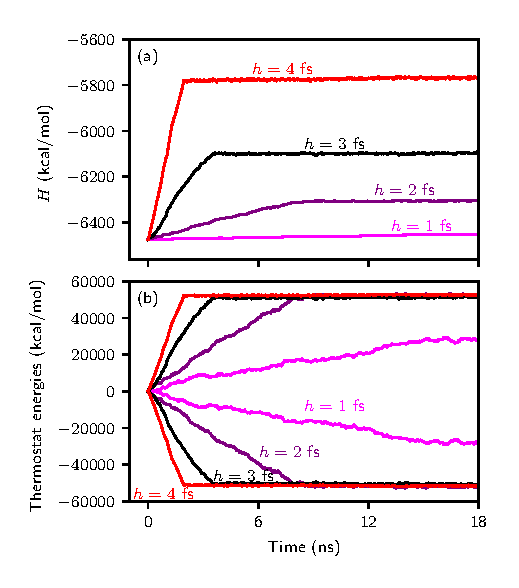
\includegraphics{Figures/numerical_stability.eps}
    \caption{Total extended energy of 903 TIP3P\cite{Jorgensen_1983} water molecules obtained by NVT MD simulations with different time
step sizes, employing (a) the proposed method represented by Eq. ; (b) our implementation for rigid bodies of the integrator due to Martyna \textit{et al.} \cite{Martyna_1996} and (c) the NVT method introduced by Kamberaj \textit{et al.} \cite{Kamberaj_2005}.Energy of thermostats for 903 TIP3P\cite{Jorgensen_1983} water molecules obtained by NVT MD simulations with different time
step sizes, employing the NVT method introduced by Kamberaj \textit{et al.} \cite{Kamberaj_2005}.}
	\label{fig:num_stab}
\end{figure}

\subsection*{Effect of Discretization Errors on Equilibrium Thermodynamic Properties}

We now turn our focus to discretization errors.
In Fig.~\ref{fig:properties} we show the computed average of some thermodynamic properties as a function of $\timestep$. The simulations were carried out at a specified temperature of T = 298 K and the analyzed quantities correspond to temperature ($T$), potential energy ($U$) and virial ($W$) per molecule, as well as the constant-volume heat capacity ($C_v$). The temperature was calculated from the kinetic energy assuming equipartition, ie $2 \langle K \rangle = (6N -3) k_b T$.
The lines are a guide for the eye. 
Also, the horizontal dotted lines (black) help to visualize the departure of the computed averages with increasing $\timestep$.
They correspond to the results obtained employing $h$ = 1 fs in the numerical scheme proposed in this paper, which from now on will be referred as ``This work''.
In addition, we have included the results of applying our proposal but using the approximate solution of rotation due to Miller \textit{et al.} \cite{Miller_2002}, which is denoted as ``This work (NO-SQUISH)''.
Despite the non-equilibrium process ocurring within the thermostats, it is worth showing the results obtained with the method of Kamberaj \textit{et al.} \cite{Kamberaj_2005}, because that is not the only problematic issue related to the method in question.
Particularly, from Fig.~\ref{fig:properties} (a) we note that the simulated temperature decreases systematically with $\timestep$.
This kind of behavior is observed in NVE simulations\cite{Davidchack_2009,Silveira_2017}, reflecting that the factorization employed in Kamberaj \textit{et al.} \cite{Kamberaj_2005} in not suitable. 
As a result of this inefficient temperature control, the potential energy and virial are not severely influenced by $\timestep$ as they are in the scheme of Martyna \textit{et al.} \cite{Martyna_1996} (see Fig.~\ref{fig:properties} (b) and (c)).
From Fig.~\ref{fig:properties} it becomes clear that our method yields significantly improved results: we are able to simultaneously reproduce the specified temperature and the other thermodynamic properties. 
This is true also for the results corresponding to the use of the NO-SQUISH method\cite{Miller_2002} in the NVE part of the integrator.
Mathematically, the derivation of the refined Hamiltonian was facilitated by the fewer number of operators associated with the exact solution of rotation. However, the accuracy of the approximate solution is very high for the time step sizes considered\cite{Silveira_2017} and this explains the good agreement.

With the aim of highlighting the importance of reweighting, in Table~\ref{table:reweight} we present the calculated temperature and potential energy for each $\timestep$ before and after applying Eq.~\ref{eq:reweighting}. The ``refined'' temperature $\modified{T}$ was calculated by means of the generalized equipartition theorem, given by Eq.~\ref{eq:equipartition}. Of course, as $\modified{T}$ is indirectly controlled by means of Eq.~\ref{eq:thermostat_force}, it is expected to reproduce the specified temperature. Indeed, for time step sizes up to, the agreement is excelent. Note that in the abscence of reweighting, the calculated temperatures are notably influenced by $h$. The free energy difference between the sampled state $\modified{\Ham{}}$ and the state we would like to sample, represented by the physical Hamiltonian $\Ham{}$. As expected, the $\Delta F$ is small, as it should be 
Note that a small, still clearly influencing systematic error is present in our scheme.

\begin{table*}
	\caption{Effect of the time-step size on .... of 903 TIP3P\cite{Jorgensen_1983} water molecules in NVT MD simulations employing the unsplit solution for free rotations, given by the numerical schemes. uncertainties in free energy never exced 1e-4}
    \label{table:reweight}
    \sisetup{
table-number-alignment = center
}
    \begin{tabular}{SS[separate-uncertainty,table-figures-uncertainty = 2]S[separate-uncertainty,table-figures-uncertainty=2]S[separate-uncertainty,table-figures-uncertainty= 1,table-figures-decimal=4]S[separate-uncertainty,table-figures-uncertainty= 1]S[separate-uncertainty,table-figures-uncertainty= 1,table-figures-decimal=4]S}
     & &  \multicolumn{2}{c}{no reweighting} & \multicolumn{2}{c}{after reweighting} & \\
     \cmidrule[0.5mm](lr){3-4} \cmidrule[0.5mm](lr){5-6}
     $\timestep$ & $\modified{T}$  & $T$  & {$\langle U/N \rangle$}  & $T$ & {$\langle U/N \rangle$}   & {$\Delta F$} \\
        $\text{(fs)}$  & $\text{(K)}$ & $\text{(K)}$ & $\text{(kcal/mol)}$  & $\text{(K)}$ & $\text{(kcal/mol)}$ & $\text{(kcal/mol\,N)}$ \\
	1 & 298.00(1) & 297.71(1) & -9.1015(3) & 298.00(1) & -9.1028(3) & -0.001 \\
	2 & 297.99(1) & 296.82(1) & -9.0970(3)  & 297.98(1)  & -9.1024(3) & -0.006 \\
	3 & 297.98(1) & 295.38(1) & -9.0885(3) & 297.92(1) & -9.1005(3) & -0.013 \\
	4 & 298.01(1) & 293.49(1)& -9.0764(3) & 297.85(3) & -9.0969(3) & -0.022 \\
	5 & 297.99(1)& 291.13(1)& -9.0577(3) & 297.6(2) & -9.091(1) & -0.033 \\
    6 & 298.00(1) & 288.46(1) & -9.0314(3) & 298.8(3) & -9.075(3) &  -0.045 \\
	7 & 297.99(1) & 285.57(1) & -8.9944(3)  & 295.0(5)  & -9.040(4) & -0.056 \\

	\end{tabular}
\end{table*}

To end this section,  Kinetic Energy Partition

\begin{figure*}
	\includegraphics{Figures/thermodynamic_properties.eps}
	\caption{Effect of the time-step size on the thermodynamic properties and of 903 TIP3P\cite{Jorgensen_1983} water molecules in NVT MD simulations employing...}
	\label{fig:properties}
\end{figure*}

\begin{figure*}
	\includegraphics{Figures/energy_partition.eps}
\end{figure*}

\begin{table*}
	\caption{Effect of the time-step size on .... of 903 TIP3P\cite{Jorgensen_1983} water molecules in NVT MD simulations employing the unsplit solution for free rotations, given by the numerical schemes....}
	\label{table:check_ens}
	\sisetup{table-number-alignment = center}
    \begin{tabular}{SS[separate-uncertainty,table-figures-uncertainty = 2]SS[separate-uncertainty,table-figures-uncertainty= 1]SS[separate-uncertainty,table-figures-uncertainty= 1]S}
	{$\timestep$} & {estimated $\Delta T$} & {$\sigma$ deviations}  & {estimated $\Delta T$}  & {$\sigma$ deviations}  &    {estimated $\Delta T$}  & {$\sigma$ deviations} \\
	{(fs)} & {(K)} &   & {(K)}  &  & {(K)}  & \\
			\hline
			\multicolumn{7}{c}{``This work (Unsplit)''}\\
1.0	& 3.02(2) & 1.07 & & & &  \\
2.0 & 3.02(2) & 0.81 & & & &  \\
3.0 & 2.98(2) & 0.73 & & & &  \\
4.0 & 3.01(2) & 0.41 & & & &  \\
5.0 & 3.02(2) & 0.79 & & & &  \\
6.0 & 3.03(3) & 1.23 & & & &  \\
7.0 & 2.98(2) & 0.74 & & & &  \\
            \hline
			\multicolumn{7}{c}{Martyna \textit{et al.} \cite{Martyna_1996}}\\
1.0	& 2.98(2) & 0.66 & 3.01(2) & 0.49 & 2.96(3) & 0.90 \\
2.0 & 2.98(2) & 0.73 & 2.99(2) & 0.03 & 3.02(3) & 0.66 \\
3.0 & 2.95(2) & 2.33 & 3.01(2) & 0.65 & 2.91(3) & 2.47 \\
4.0 & 3.00(2) & 0.01 & 3.01(2) & 0.72 & 2.92(3) & 2.19  \\
5.0 & 2.93(2) & 3.05 & 3.01(2) & 0.70 & 2.94(3) & 1.58  \\
6.0 & 2.92(2) & 3.87 & 3.00(2) & 0.22 & 2.91(3) & 2.76  \\
7.0 & 2.89(2) & 5.35 & 3.02(1) & 1.33 & 2.87(2) & 4.33  \\
            \hline
			\multicolumn{7}{c}{Kamberaj \textit{et al.} \cite{Kamberaj_2005}}\\
1.0	& 2.97(2) & 1.16 & 2.99(2) & 0.16 & 2.89(3) & 2.84  \\
2.0 & 3.00(2) & 0.02 & 3.02(2) & 0.99 & 2.00(4) & 0.25  \\
3.0 & 2.99(4) & 0.18 & 3.08(4) & 4.09 & 3.1(1) & 1.17  \\
4.0 & 2.92(8) & 0.99 & 3.12(2) & 6.01 & 2.8(2) & 0.95  \\
5.0 & 3.02(5) & 0.40 & 3.2(2)  & 9.50 &  2.9(1) & 0.28  \\
6.0 & 3.14(5) & 2.69 & 3.29(2) & 14.68 & 3.21(7) & 2.90  \\
7.0 & 3.03(4) & 0.73 & 3.35(2) & 17.37 & 2.99(6) & 0.16  \\
    \end{tabular}
\end{table*}
%It is not the purpose of this work to propose an optimal factorization scheme for the NVT dynamics, but rather to prove that a unique thermostat chain is capable of maintaining the average temperature at its specified value while providing the proper sampling of the canonical ensemble.
%First we present some results as first mented.
%That is, the proposed methods coupling to a single thermostat, while in Kamberaj the translational and rotational degrees of freedom are separatedly coupled.
%In Table~\ref{table:new_results}, it can be seen that the integrators proposed here, which are represented by the Eqs.~\eqref{eq:trotter_splitting_NHC} and ~\eqref{eq:modified_splitting}, systemcatically achive the specifed temperature, regardless of the time step size.
%By contrast, the numerical solver introduced by Kamberaj and co-workers\cite{Kamberaj_2005} fails to yield the specified temperature for even the smaller time step size of 1 fs.
%Resultados sobre o checkensemble: 

%checkensemble:We report the results corresponding to that method, and since it is instructive to have a graphical insight, we also show some figures of the linear fitting.
%Given that the potential and kinetic energies are separable, the analysis can be made separately as follows.This last approach does not involve any binning of the energies, hence no discretization error is present.
%m-b distribution valid when equipartition of energy is satisfied.

%Recalling that in the NVT dynamics the conserved quantity is the extended energy $H$ of Eq.~\eqref{eq:H_nvt}, in Table~\ref{table:new_results_2} we report the energy drift, denoted by $R$, as the the rate of change of $H$ (kcal/mol) with time (ns), which is the angular coefficient obtained from linear regression fitting  between those variables.
%Except for the case of $\Delta$ = 1 fs, there is also a clear correspondece between an incresing $R$ with the failure in keeping the temperature at its specified value.

%In Fig.~\ref{fig:checkensemble} we show the result from the linear regression analysis for the potential energies sampled using Eq.~\eqref{eq:trotter_splitting_NHC}.
%In figure legends we show the averages temperatures simulated.
%It can be seen that the mentioned algorithm generates a distribution consistent with the canonical ensemble, and that is also true for the kinetic energies.
%Likewise, in Fig.~\ref{fig:mbdistribution} we observe a good correspondence between the kinetic energy distribution at $T= 304.99 K$ and the corresponding Maxwell-Boltzmann distribution We arrive at the same conclusions for the approach given by Eq.~\eqref{eq:modified_splitting}.

%Finally, in Table~\ref{table:ensemblevalidation} we present the results of the maximum likelihood approach applied for both NVT integration schemes.
%It can be seen that the deviations from the true slope, $\timestep$ = 8.970~K, are less than $1\sigma$.
%This means that effectively, the sampled values do not deviate from the correct distribution to a statistically noticeable level.

\section{Concluding Remarks}
\label{sec:conclusion}
Nevertheless, as will be shown in the forthcoming section, those numerical schemes successfully achieve the specified temperature and an acceptable long-term conservation of the extended energy $H$.

by contrast

\begin{acknowledgement}
	The authors acknowledge the financial support provided by Petrobras (project code CENPES 16113).
\end{acknowledgement}

\appendix

\section{Backward Error Analysis}
\label{sec:rigid body shadow hamiltonian}

For two non-commutative Liouville operators $\Liu A$ and $\Liu B$ and a real constant $\timestep$, the symmetric Baker-Campbell-Hausdorff (BCH) formula can be expressed as \cite{Hairer_2006}
\begin{equation}
\label{eq:symmetric BCH}
\begin{split}
&e^{\frac{\timestep}{2} \Liu B} e^{\timestep \Liu A} e^{\frac{\timestep}{2} \Liu B} = \\
&= e^{\timestep (\Liu A + \Liu B) + \frac{\timestep^3}{24} \left[2 \Liu A + \Liu B,[\Liu A,\Liu B]\right] + \mathcal{O}(\timestep^5)},
\end{split}
\end{equation}
where $[X,Y]$ is the commutator of operators $X$ and $Y$, defined as $[X,Y] = XY - YX$.
The remaining terms of the infinite series involve ever-deepening, nested commutators \cite{Hairer_2006}.

Let us now represent the operators $\Liu A$ and $\Liu B$ using Poisson brackets involving Hamiltonians $\Ham A$ and $\Ham B$, that is, $\Liu A = \{\circ,\Ham A\}$ and $\Liu B = \{\circ,\Ham B\}$.
By employing the properties of anti-commutativity and Jacobi identity \cite{Hairer_2006}, we can deduce that
\begin{align*}
[\Liu A,\Liu B] &= \{\{\circ,\Ham B\},\Ham A\} - \{\{\circ,\Ham A\},\Ham B\} = \\
&= -\{\Ham A,\{\circ,\Ham B\}\} - \{\Ham B,\{\Ham A,\circ\}\} = \\
&= \{\circ,\{\Ham B,\Ham A\}\} = \\
&= \{\circ,{\Liu A} {\Ham B}\}.
\end{align*}

This means that the commutator $[\Liu A,\Liu B]$ is, in fact, a new Liouville operator $\Liu C$ whose associated Hamiltonian is $\Ham C = {\Liu A}{\Ham B}$.
By applying this procedure recursively, we can rewrite the right-hand side of Eq.~\eqref{eq:symmetric BCH} as $e^{\timestep \Liu S}$, where $\Liu S$ is the Liouville operator whose associated Hamiltonian is
\begin{equation*}
\label{eq:general shadow hamiltonian}
\modified{\Ham{}} = \Ham A + \Ham B + \frac{h^2}{24} (2 \Liu A + \Liu B){\Liu A}{\Ham B} + \mathcal{O}(h^4).
\end{equation*}

Therefore, a splitting method meant to approximately reproduce the dynamics of a system with Hamiltonian $\Ham{} = \Ham A + \Ham B$ will, in fact, reproduce exactly (putting round-off issues aside) the dynamics of another system with Hamiltonian $\modified{\Ham{}}$ as above.
In the literature, $\modified{\Ham{}}$ is usually referred to as a shadow Hamiltonian.

In the development that follows, we consider a single rigid body and, in the end, we generalize the result for a system of rigid bodies.

For the splitting introduced in Section~\ref{sec:nve}, $\Ham A = K(\vt p, \vt q, \vt \pi)$ and $\Ham B = U(\vt r, \vt q)$ with the corresponding Liouviller operators $\Liu{A} = \tr{K_{\vt p}}\diff{}{\vt r} + \tr{K_{\vt \pi}}\diff{}{\vt q} - \tr{K_{\vt q}}\diff{}{\vt \pi}$ and $\Liu{B} = -\tr{U_{\vt r}}\diff{}{\vt p} - \tr{U_{\vt q}}\diff{}{\vt \pi}$, with $K_{x}$ and $U_{x}$ being the gradient of the kinetic and potential energies, respectively.
We first obtain $\Liu A \Ham B = \tr{K_{\vt p}} U_{\vt r} + \tr{K_{\vt \pi}} U_{\vt q}$, and we find that
\begin{align*}
\Liu A \Liu A \Ham B &= \tr{K_{\vt p}} U_{\vt r \vt r} K_{\vt p}
+ 2 \tr{K_{\vt \pi}} U_{\vt r \vt q} K_{\vt p}
+ \tr{K_{\vt \pi}} U_{\vt q \vt q} K_{\vt \pi} \\
&+ \tr{K_{\vt \pi}} K_{\vt \pi \vt q} U_{\vt q}
- \tr{K_{\vt q}} K_{\vt \pi \vt \pi} U_{\vt q},
\end{align*}
where the fact that $\tr{U_{\vt q \vt r}} = U_{\vt r \vt q}$ has been exploited.
As reported in Ref.~\citenum{Silveira_2017}, the identity $\tr{\mt B}(\vt q) {\vt \pi} = -\tr{\mt B}(\vt \pi) {\vt q}$ is useful for performing differentiations.
The first-order derivatives of $K$ with respect to $\vt p$, $\vt q$, and $\vt \pi$ are, respectively,
\begin{align*}
&K_{\vt p} = {\mt M}^{-1} {\vt p}, \\
&K_{\vt q} = -\frac{1}{2} {\mt B}(\vt \pi) {\vt \omega}, \; \text{and} \\
&K_{\vt \pi} = \frac{1}{2} {\mt B}(\vt q) {\vt \omega},
\end{align*}
where $\vt \omega = \frac{1}{2} {\mt I}^{-1} \tr{\mt B}(\vt q) \vt \pi = -\frac{1}{2} {\mt I}^{-1} \tr{\mt B}(\vt \pi) \vt q$.\cite{Silveira_2017} Hence,
\begin{gather*}
\tr{K_{\vt p}} U_{\vt r \vt r} K_{\vt p} = \tr{\vt p} {\mt M}^{-1} U_{\vt r \vt r} {\mt M}^{-1} {\vt p}, \\
\tr{K_{\vt \pi}} U_{\vt r \vt q} K_{\vt p} = \frac{1}{2} \tr{\vt \omega} \tr{\mt B}(\vt q) U_{\vt r \vt q} {\mt M}^{-1} {\vt p}, \\
\tr{K_{\vt \pi}} U_{\vt q \vt q} K_{\vt \pi} = \frac{1}{4} \tr{\vt \omega} \tr{\mt B}(\vt q) U_{\vt q \vt q} {\mt B}(\vt q) \vt \omega.
\end{gather*}

As $\diff{\tr{\vt \omega}}{\vt \pi} = \frac{1}{2} {\mt B}(\vt q) {\mt I}^{-1}$, the second-order derivative of $K$ with respect to $\vt \pi$ turns out to be
\begin{equation*}
K_{\vt \pi \vt \pi} = \frac{1}{4} {\mt B}(\vt q) {\mt I}^{-1} \tr{\mt B}(\vt q).
\end{equation*}

Pre-multiplication by $\tr{K_{\vt q}}$ will introduce a product $\tr{\mt B}(\vt \pi) {\mt B}(\vt q)$, which has been shown in Ref.~\citenum{Silveira_2017} to be equal to ${\mt S}\left( \tr{\mt B}(\vt \pi) {\vt q} \right) = -2 {\mt S}({\mt I} {\vt \omega})$, where the operator ${\mt S}(\cdot)$ builds a skew-symmetric matrix from the entries of a vector.
In addition, post-multiplication by $U_{\vt q}$ will introduce a product $\tr{\mt B}(\vt q) U_{\vt q}$, which is equal to $-2 {\vt \tau}^b$, where ${\vt \tau}^b$ is the body-fixed frame representation of the torque.
Then, the fact that ${\mt S}(\vt x) {\vt y} = -{\mt S}(\vt y) {\vt x}$ leads to
\begin{equation*}
\tr{K_{\vt q}} K_{\vt \pi \vt \pi} U_{\vt q} = \frac{1}{2} \tr{\vt \omega} {\mt S}({\mt I}^{-1} {\vt \tau}^b) {\mt I} {\vt \omega} = 0,
\end{equation*}
which is a null term as it corresponds to the quadratic form of a skew-symmetric matrix.
Another helpful identity taken from Appendix B of Ref.~\citenum{Silveira_2017} is ${\mt B}(\vt q){\vt \omega} = ( \sum_{k=1}^3 \omega_k \hat{\mt B}_k ) \vt q$, where each $\hat{\mt B}_k$ is a skew-symmetric permutation matrix (i.e.
$\tr{\hat{\mt B}}_k = -\hat{\mt B}_k$).
This allows us to obtain
\begin{align*}
K_{\vt \pi \vt q} &= \frac{1}{2} (\diff{\tr{\vt \omega}}{\vt q}) \tr{\mt B}(\vt q) + \frac{1}{2} \sum_{k=1}^3 \omega_k \tr{\hat{\mt B}}_k = \\
&= -\frac{1}{4} {\mt B}(\vt \pi) {\mt I}^{-1} \tr{\mt B}(\vt q) - \frac{1}{2} \sum_{k=1}^3 \omega_k \hat{\mt B}_k.
\end{align*}

Pre-multiplication by $\tr{K_{\vt \pi}}$ and post-multiplying $U_{\vt q}$, followed by some algebraic transformations, ultimately lead to
\begin{equation*}
\tr{K_{\vt \pi}} K_{\vt \pi \vt q} U_{\vt q} = -\frac{1}{2} \tr{\vt \omega} \tr{\mt S}({\mt I}^{-1} {\vt \tau}^b) {\mt I} {\vt \omega} + \frac{1}{2} \tr{\vt \omega} {\mt S}({\vt \tau}^b){\vt \omega}.
\end{equation*}
Both terms in the right-hand side of the equation above are identically null. 
Now, we are able to evaluate $\Liu A \Liu A \Ham B $, which is
\begin{align*}
\Liu A \Liu A \Ham B = &\tr{\vt p} {\mt M}^{-1} U_{\vt r \vt r} {\mt M}^{-1} {\vt p} + \tr{\vt \omega} \tr{\mt B}(\vt q) U_{\vt r \vt q} {\mt M}^{-1} {\vt p}
+ \\
&\frac{1}{4} \tr{\vt \omega} \tr{\mt B}(\vt q) U_{\vt q \vt q} {\mt B}(\vt q) \vt \omega.
\end{align*}
The remaining term to obtain $H_s$ is simply given by 
\begin{align*}
\Liu B \Liu A \Ham B &= -\tr{U_{\vt r}} \tr{K_{\vt p \vt p}} U_{\vt r} - \tr{U_{\vt q}} \tr{K_{\vt \pi \vt \pi}} U_{\vt q} = \\
&= -\tr{\vt F} {\mt M}^{-1} {\vt F} - \tr{\vt \tau}_b {\mt I}^{-1} {\vt \tau}_b.
\end{align*}

As will become clear below, it is convenient to rewrite the total kinetic energy of the original system, Eq.~\eqref{eq:kinetic energy}, as a quadratic form
\begin{equation*}
K = \frac{1}{2} \tr{ \left[\begin{array}{c} \vt p \\ \vt \pi \end{array}\right]} {\mt \Omega}(\vt q) \left[\begin{array}{c} \vt p \\ \vt \pi \end{array}\right],
\end{equation*}
where $\mt \Omega$ is a symmetric, block-diagonal matrix of size $7N \times 7N$ defined as
\begin{equation*}
{\mt \Omega} = \left[\begin{array}{cc}
{\mt M}^{-1} & \mt 0 \\
\mt 0 & \frac{1}{4} {\mt B}(\vt q) {\mt I}^{-1} \tr{\mt B}(\vt q)
\end{array}\right].
\end{equation*}

We now proceed to show the final expression of $H_s$, which results from grouping the terms corresponding to forces and torques in the \textit{modified} potential energy $\tilde{U}$, given by
\begin{equation*}
\modified U = U - \frac{\timestep^2}{24} \left( \tr{\vt F} {\mt M}^{-1} {\vt F} + \tr{\vt \tau} \tr{\mt A} {\mt I}^{-1} {\mt A} {\vt \tau} \right).
\end{equation*}
while the remaining terms can be recast in a compact matrix, as follows
\begin{equation*}
\modified K = \frac{1}{2} \tr{ \left[\begin{array}{c} \vt p \\ \vt \pi \end{array}\right]} \modified{\mathbf \Omega}(\vt r, \vt q) \left[\begin{array}{c} \vt p \\ \vt \pi \end{array}\right],
\end{equation*}
where
\begin{equation*}
\tilde{\mt \Omega} = {\mt \Omega} + \frac{\timestep^2}{6} \left( {\mt \Omega} {\mt U}_{\vt x \vt x} \tr{\mt \Omega} \right)
\end{equation*}
and
\begin{equation*}
{\mt U}_{\vt x \vt x} = \left[\begin{array}{cc}
U_{\vt r \vt r} & U_{\vt r \vt q} \\
U_{\vt q \vt r} & U_{\vt q \vt q}
\end{array}\right].
\end{equation*}

Finally, we have that
\begin{equation*}
\Ham S = \frac{1}{2} \tr{\left[\begin{array}{c} \vt p \\ \vt \pi \end{array}\right]} \tilde{\mt \Omega} \left[\begin{array}{c} \vt p \\ \vt \pi \end{array}\right] + \tilde{U} + \mathcal{O}({\timestep}^4),
\end{equation*}

Although $\modified{\mathbf \Omega}$ is still symmetric, it is no longer a block-diagonal matrix like $\mt \Omega$, due to the inter-body interactions accounted for in $U(\vt r, \vt q)$ and to the dependency of forces and torques on both positions and orientations.
As a result, the modified kinetic energy cannot, in principle, be split into independent translational and rotational contributions.

\suppinfo

\begin{table}
	\caption{Effect of the time-step size on .... of 903 TIP3P\cite{Jorgensen_1983} water molecules in NVT MD simulations employing the unsplit solution for free rotations, given by the numerical schemes.}
    \label{table:stability_martyna}
    \begin{tabular}{SS[table-number-alignment = center,table-figures-exponent = 1]S[table-number-alignment = center,table-figures-exponent = 1]}
     & \multicolumn{2}{c}{Martyna \textit{et al.} \cite{Martyna_1996}}  \\
     \cmidrule[0.5mm](lr){2-3} 
     $\timestep$ $\text{(fs)}$  & $\modified{H}$  & $\modified{\Ham{}}$     \\
	1 &  -1.6e-2  & 4.5e-3\\
	2 & 9.5e-2 & 1.4e-1\\
	3 & 2.8e-1 & 5.6e-2\\
	4 & 1.1e0 & 5.6e-2\\
	5 & 3.3e0 & -3.7e-2\\
    6 & 6.1e1 & 6.9e-2 \\
	7 & 9.8e2 & -3.6e-3 \\
	8 & 1.1e4 & 1.8e-2 \\
	9 & 7.5e4 & 3.8e-3 \\
	10 & 3.3e5 & 1.9e-2  \\
	\end{tabular}
\end{table}

\bibliography{rigid_bodies}
\end{document}
